\documentclass[11pt]{article}

\usepackage[utf8]{inputenc}
\usepackage[T1]{fontenc}
\usepackage[english]{babel}
\usepackage{amssymb}
\usepackage{color}
\usepackage{wrapfig}
\usepackage{lipsum}
\usepackage{amsmath}
\usepackage[enable]{easy-todo} % change to disable to hide todo's
\usepackage[hidelinks]{hyperref}
\usepackage{url}

%\usepackage[
%backend=biber,
%style=alphabetic,
%sorting=ynt
%]{biblatex}



% margins
\usepackage{geometry}
\geometry{
	a4paper,
	total={170mm,257mm},
	left=14mm,
	right=14mm,
	top=18mm,
}
\font\myfont=cmr12 at 15pt


%\newcommand{\todo}{{\color{red}{\textbf{TODO }}}}


\title{\vspace{-2.5cm}{\myfont Report Project 2: BDAP [B-KUL-H00Y4A]}}
\author{Andreas Hinderyckx - r0760777}
\date{\vspace{-.2cm}} 

\usepackage{graphicx}
\usepackage{caption}

%\addbibresource{sources.bib}

\begin{document}

%\section*{Report Project 2: BDAP [B-KUL-H00Y4A]\\ Andreas Hinderyckx}
\maketitle

\vspace{-1.5cm}
%\listoftodos
\subsection*{Part 1: Trip Length Distribution}
The pure Java implementation was implemented by reading each line of the \texttt{.trips} file, calculating the distance between the start and end coordinates of that trip using a flat-surface formula\footnote{\url{https://en.wikipedia.org/wiki/Geographical_distance\#Flat-surface_formulae}} and writing the result to the output file. The Spark implementation reads the \texttt{.trips} file as a csv using the \texttt{SparkSession}, and parallelizes it into an RDD using the \texttt{SparkContext}. Next, the distances are calculated by applying a \texttt{Map} transformation to the read data. Finally, the data is written to an output file.

The run time of the pure Java-implementation is 0.927 seconds, whereas the Spark implementation took 5.114 seconds. The pure Java-implementation is about 5 times as fast: this is as expected, as the Spark implementation introduces quite some overhead by setting up the \texttt{SparkContext}, converting the data to an RDD, dividing the RDD into logical partitions, creating the Directed Acyclic Graph (DAG) to schedule tasks and orchestration of worker nodes... \footnote{\url{https://www.ibm.com/cloud/learn/apache-spark\#toc-how-apache-VZl4w8Yx}} The performance gain achieved by parallelizing the task in-memory does not outweigh the introduced overhead; thus, the pure Java implementation is indeed faster for small files such as \texttt{2010\_03.trips}.
The normalized histogram of the trip durations is shown in figure \ref{fig:tripLenghts}, where trips with a length $\geq20$ km are collected in the last bin. When seeking to minimize the sum of squared errors, the data is best approximated by the \texttt{sciPy} Folded Cauchy distribution\footnote{\url{https://docs.scipy.org/doc/scipy/reference/generated/scipy.stats.foldcauchy.html}}, with parameters $\approx$ (c: 1.28, location: -4.58e-10, scale: 1.28), which achieves a sum of squared errors $\approx 0.037$. This approximation is also shown in figure \ref{fig:tripLenghts}


%\begin{figure}
%	\centering
%	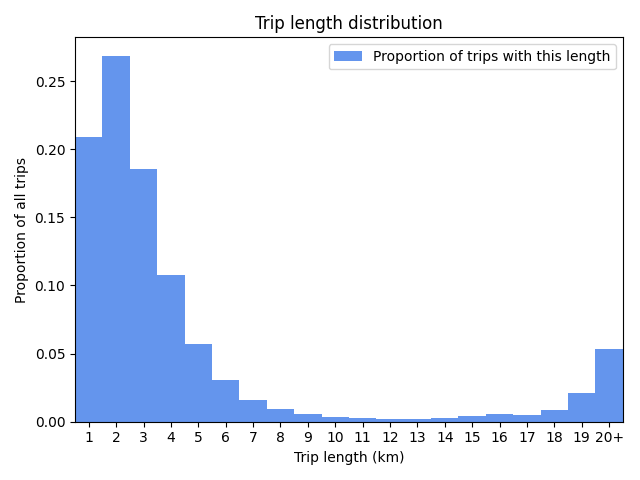
\includegraphics[width=.5\linewidth]{./img/trip_distribution.png}
%	\caption{Distribution of trip lengths}
%	\label{fig:tripLengths}
%\end{figure}

\begin{figure}
	\begin{minipage}{.48\textwidth}
		\centering
		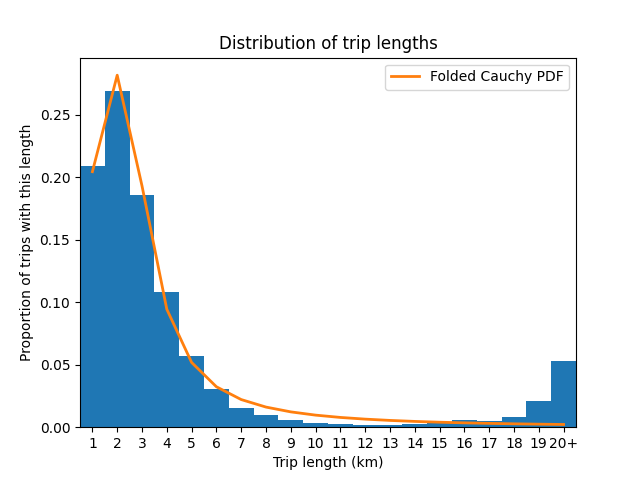
\includegraphics[width=1.2\linewidth]{./img/trip_distribution_with_dist.png}
		\caption{Distribution of trip lengths}
		\label{fig:tripLenghts}
	\end{minipage}\hfill
	\begin{minipage}{.48\textwidth}
		\centering
		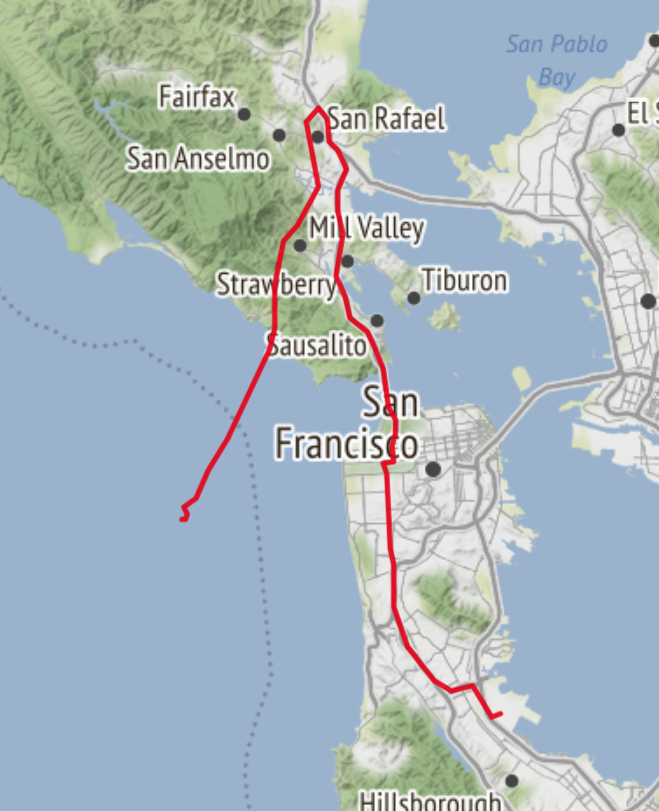
\includegraphics[width=.7\linewidth]{./img/sea-trip1.png}
		\caption{An airport trip ({\color{red} red} line) that ends up in an erroneous location}
		\label{fig:seatrip}
	\end{minipage}
\end{figure}

\vspace{-.3cm}
\subsection*{Part 2: Computing Airport Revenue}

\textbf{Identifying erroneous GPS points}
The first technique used to identify erroneous GPS points is to verify whether the calculated speed of a segment is smaller than 200 km/h. A lower speed limit was not chosen, as GPS results may be imprecise at times, which could cause valid but slightly inaccurate trips to be invalidated as well. Segments that don't contain 9 comma separated fields, or contain NULL-values are rejected as well, for example: \\
\hspace{-2cm}\verb|2876,'2010-03-12 14:14:54',37.75116,-122.39468,'E',NULL,NULL,NULL,NULL|.
Furthermore, it was apparent that quite some GPS points were located in the sea, to the West of San Francisco. One can reject these points either in the mapper, or in the reducer. 

% Example of two the second segment being a subset of the first:
% 1007,'2010-03-10 09:01:07',38.08841,-121.27446,'E','2010-03-10 09:03:07',38.08192,-121.2613,'M'
% 1007,'2010-03-10 09:02:07',38.08463,-121.26412,'M','2010-03-10 09:03:07',38.08192,-121.2613,'M'

% Example of unfinished trip on edge of data, and the next segment which is of a different TaxiID
% 1065,'2010-03-3123:59:56',37.79014,-122.3911,'M','2010-04-0100:10:50',37.79598,-122.42184,'M'
% 1074,'2010-03-0100:27:41',37.76485,-122.42274,'E','2010-03-0100:28:42',37.76338,-122.42009,'M'

To implement the former, two coordinates were handpicked to create a rough approximation of the coastline. Based on the cross product's properties, points to the west of this coast line were rejected. This check detected roughly 1500 points, but did hurt performance, however (see below). Therefore, the latter option was chosen: points were rejected in the reducer by checking whether they formed an airport trip, and by checking the speed of each segment as mentioned. This approach rejects trips containing sudden large jumps to erroneous coordinates, and thus eliminates the majority of erroneous trips.
Extra checks (e.g.verifying the elapsed time between two subsequent records, or verifying whether their coordinates properly chain up) were unnecessary as these detected segments are already invalidated by the previous checks. Other examples of segments that lead to erroneous calculations, are those that take place during another segment's time-span:

\hspace{-1.5cm}\verb|1007,'2010-03-10 09:01:07',38.08841,-121.27446,'E','2010-03-10 09:03:07',38.08192,-121.2613,'M'|
% this enter is needed in order for the second hspace to take affect!

\hspace{-1.5cm}\verb|1007,'2010-03-10 09:02:07',38.08463,-121.26412,'M','2010-03-10 09:03:07',38.08192,-121.2613,'M'|

and those that are part of a trip which doesn't end during the period within which the data was recorded. Segments pertaining to the first case are skipped in the reducer to prevent doubly counted distances. The corresponding trip is still counted as a valid trip. Trips belonging to the second case are detected by comparing the \texttt{TaxiID} to that of the previous segment. As we do not have access to the complete data of these trips, it was chosen not to count these trips as valid ones.

Finally, there are also airport trips which still pass the checks mentioned above, but start in the airport and end up in an erroneous location (the ocean): figure \ref{fig:seatrip} shows an example of such a trip. There are only three trips that satisfy these conditions, which together
make up about $0.002\%$ of the total revenue. Roughly speaking, at most 50\% of the distance traveled in each of these trips is effectively erroneous (i.e. is located in the ocean). Thus, these edge cases account for less than $0.0009\%$ of the total revenue, which is why it was decided to count these trips as valid airport trips as well. The alternative would be to eliminate these erroneous segments in the map-phase, but we don't opt for this approach as it would:
(1) be subject to overfitting to the test data, as a precise line must be drawn which acts as a classifier for valid coordinates, and
(2) incur a significant performance penalty, as these checks would need to be conducted on every segment.
%\begin{enumerate}
%	\item be subject to overfitting to the test data, as a precise line must be drawn which acts as a classifier for valid coordinates, and
%	\item incur a significant performance penalty, as these checks would need to be conducted on every segment.
%\end{enumerate}
%\begin{wrapfigure}{R}{.3\textwidth}
%	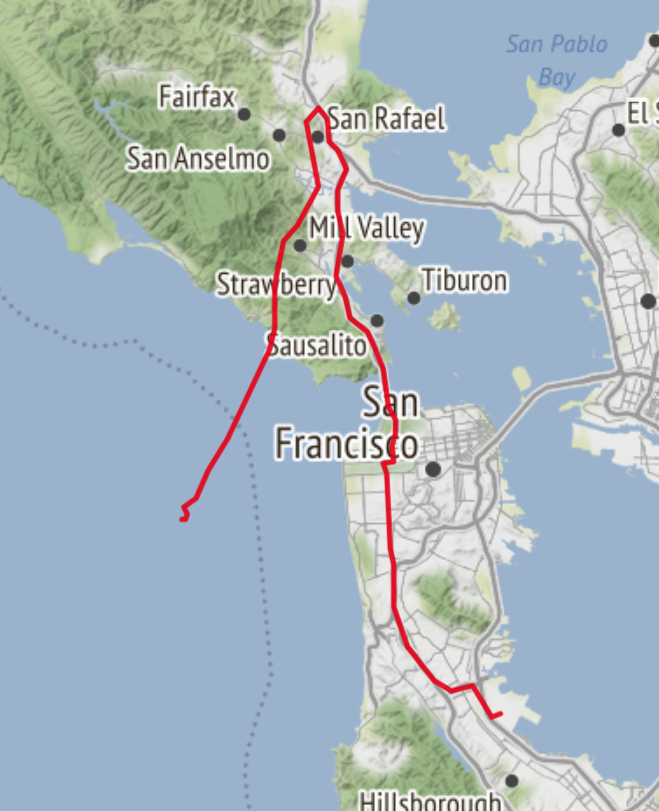
\includegraphics[width=\linewidth]{img/sea-trip1.png}
%	\caption{An airport trip that ends up in the ocean}
%	\label{img:seatrip}
%\end{wrapfigure}


%Finally, between every two segments of a trip, it is checked whether the elapsed time between the end time of the first segment and the start time of the second segment doesn't exceed three seconds.

\noindent\\\textbf{Reconstructing the trips} \\
{[NB: in what follows, a composite \texttt{key} or \texttt{value} will be respectively written as \texttt{\{key\}} or \texttt{\{value\}} to avoid confusion.]}
\noindent The trips are reconstructed in the first of the two map-reduce-processes. In the \texttt{mapper}, each segment is mapped onto a key-value pair with as key: \texttt{\{TaxiID,StartDate\}}. The custom \texttt{Comparator} implementation makes sure that the segments are primarily sorted on \texttt{TaxiID} and secondarily sorted on \texttt{StartDate}, when they are sorted by the MapReduce framework when transitioning from the \texttt{mapper} to the \texttt{reducer}. The \texttt{mapper} also rejects malformed records (see above) and doesn't map \texttt{E-E}-segments to limit network overhead, as these segments don't contribute to any trip. This already eliminates more than half of the segments. Additionally, a \texttt{Partitioner} is added to ensure that segments with the same \texttt{TaxiID} end up at the same reduce-task, and therefore end up at the same physical node to limit network overhead. Finally, a custom \texttt{GroupingComparator} implementation was added to specify which records end up in which \texttt{key, Iterable<value>} pair, received by the reducer.

Next, given the sorted order of the records, trips can be constructed during the reduce-phase. The reducer receives as input \texttt{\{TaxiID,StartDate\},Iterable<segment>} pairs. When iterating over an \texttt{Iterable<segment>}, the \texttt{reducer} looks for records that transition from the \texttt{E} state to the \texttt{M} state to initiate a trip. Subsequent \texttt{M}-\texttt{M}-records are added to the trip, until a record is encountered that transitions from the \texttt{M} state to the \texttt{E} state. During this process, the reducer rejects trips that don't satisfy the conditions explained above. To balance out, the traveled distance of \texttt{E-M} segments is included in the revenue calculation, while the distance of \texttt{M-E} segments is not included.

The second map-reduce job processes the output of the first job. This second job's mapper verifies the date format and maps each record of the output of the previous job of the form \texttt{\{StartDate ,StartCoordinates\}, \{EndCoordinates - TripRevenue\}} to a \texttt{\{Year-Month\}}, \texttt{TripRevenue} key-value pair. This way, the reducer receives as input \texttt{\{Year-Month\},Iterator<TripRevenue>} pairs, which allows it to aggregate all trips' revenues which took place during the same month to obtain the final output containing the total monthly revenues.


\textbf{Efficiency of the solution}
%\todo{Check} Due to the check that verifies whether a GPS point is not located at sea, the execution time of the program rose with a third (from $\sim9$ to $\sim12$ minutes). As these mislocated records only constitute $5\cdot 10^{-4}\%$ of the total amount of records, this is a significant performance penalty to pay for a small gain in accuracy.
As the number of mappers can't be changed directly, one must adjust the \texttt{splitSize} instead. MapReduce determines the \texttt{splitSize} (which directly determines the number of Map tasks) based on the following formula \cite{Hadoop}:
\begin{equation*}
\texttt{\text{splitSize = Math.max(minSize, Math.min(maxSize, blockSize))}}
\end{equation*}
Thus, in order to increase the number of map tasks, one must decrease the \texttt{splitSize} by decreasing the \texttt{maxSize}. To decrease the number of map tasks, one must increase the \texttt{splitSize} by increasing the \texttt{minSize} beyond the default value of \texttt{blockSize} (128Mb). The results of these actions along with memory usage are depicted in figure \ref{fig:splitSize}, which clearly shows that extremely low or high \texttt{splitSize}s lead to higher execution times, and lower split sizes lead to higher peak memory usage. The optimal choice is to take the \texttt{splitSize} around 512Mb. This is substantially higher than the default block size (128Mb), but this choice yields better efficiency as the mapper is mainly IO-bound, rather than CPU-bound. Thus, the optimal number of maps tasks is $28Gb \times 1024 \frac{Mb}{Gb} \div 512 \frac{Mb}{\text{map task}} = 56 \text{ map tasks}$. The effect of the number of reducers is shown in figure \ref{fig:nbReducers}. Here it is apparent that the number of reducers is chosen best to be slightly smaller than a multiple of 10 (which is the number of nodes in the cluster) to minimize execution time and memory usage. A possible explanation is that if a multiple of 10 is chosen and a reduce task fails, it has to wait until at least one of the other tasks is finished, whereas choosing a value slightly lower than 10 provides some slack in case of failure. Peak memory usage shows a decreasing trend, as the number of reducers increases, possibly because the reduce load is spread across more tasks. It should also be observed that picking the number of reducers around the suggested range\footnote{\hspace{.2cm}
	\begin{minipage}{.5\textwidth}
		\url{https://hadoop.apache.org/docs/current/hadoop-mapreduce-client/hadoop-mapreduce-client-core/MapReduceTutorial.html\#Reducer}
	\end{minipage}}
(in case of our cluster: 9 - 18 reducers) approximately yields the best results. Running the job with these tuned parameters (8 reducers, 28 mappers) results in a total execution time of 8-10 minutes, depending on the load on the cluster. Note: waiting time for the jobs to be scheduled for execution is not included in the execution time measurements above.


\begin{figure}
\begin{minipage}{.48\textwidth}
	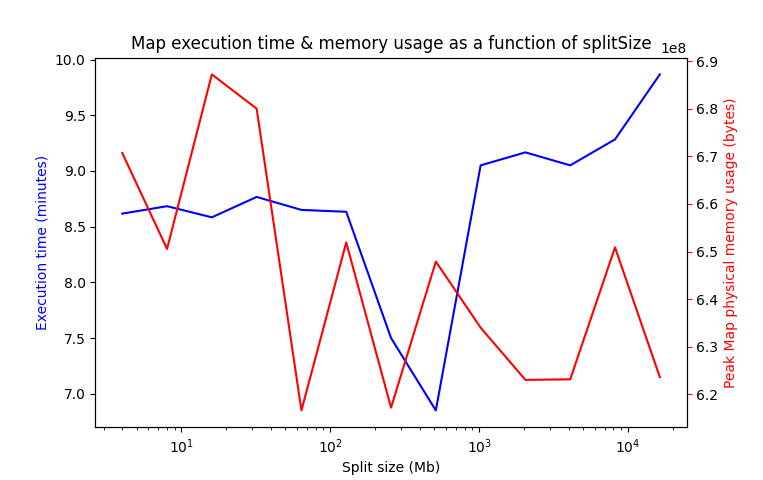
\includegraphics[width=1.1\textwidth]{./img/ExecutionMapMemoryVSMaps.png}
	\caption{Execution time and peak physical memory usage as a function of split size (on a logarithmic scale)}
	\label{fig:splitSize}
\end{minipage}\hfill
\begin{minipage}{.48\textwidth}
	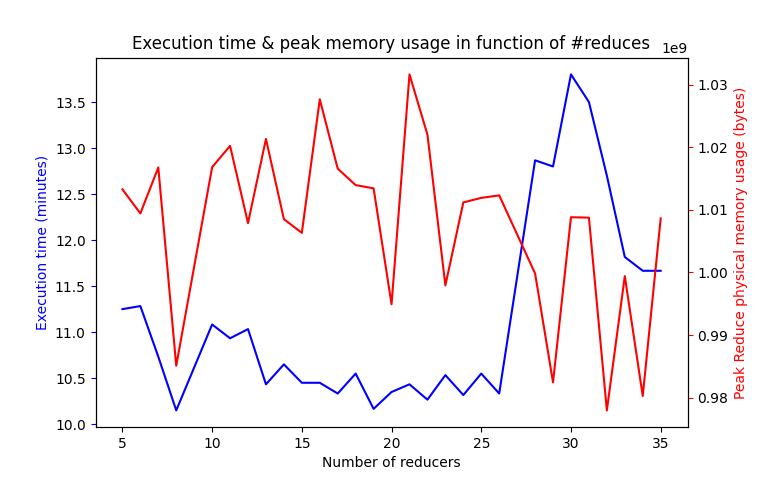
\includegraphics[width=1.1\textwidth]{./img/NewExecutionReduceMemoryVSMaps.png}
	\caption{Execution time and peak physical memory usage as a function of nb. of reducers}
	\label{fig:nbReducers}
\end{minipage}
\end{figure}

%\vspace{-.2cm}
\begin{wrapfigure}{r}{.5\textwidth}
	\vspace{-1cm}
	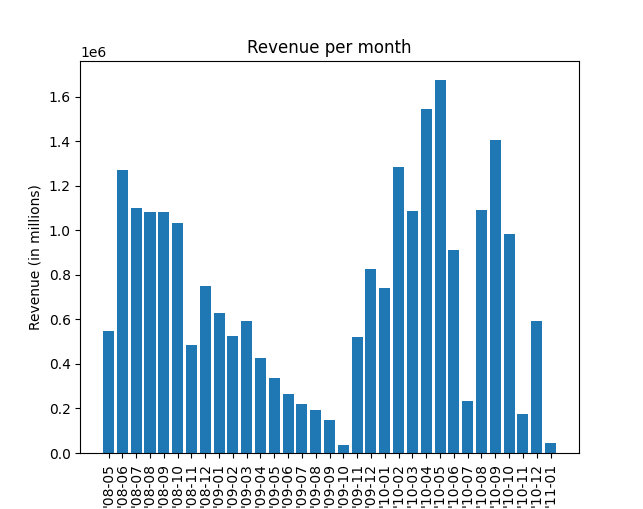
\includegraphics[width=1.2\linewidth]{./img/revenuePerMonth.png}
	\caption{Trip revenue per month}
	\label{fig:revenue}
\end{wrapfigure}

\noindent\\\textbf{Total revenue \& revenue over time}
As described above, the total revenue is aggregated per month by the map-reduce-job. These results are shown in figure \ref{fig:revenue}. It is remarkable that there are months during which almost no revenue is made; this could be due to maintenance breaks of the taxis, or due to annual leave of the taxi drivers... The approximate total revenue collected during the time-span of \texttt{all.segments} is equal to \$ $23,852,063.65$.

\vspace{-.2cm}
\bibliographystyle{acm}
\bibliography{sources}

\end{document}
